\documentclass{article}
\usepackage{graphicx}
\usepackage{caption}
\usepackage[utf8]{inputenc}

\title{Sorting Algorithms: Comparison Between Insertion, Radix, Quick and Heap Sort}
\author{Ayberk Omay Tekin}

\begin{document}
\maketitle

\section{Introduction}
In this project, we explore a sorting problem. 
The problem is to organize an array of $n$ integers in a sequence, based on total order calculated with complexity.

This paper delves into the comparison of four essential comparison based sorting algorithms: insertion sort, heap sort, quick sort, and radix sort. 
Each algorithm is examined for its efficiency and practicality in arranging data according to the specified order. 
By analyzing these methods, we aim to provide insights into their performance characteristics and optimal use cases.

\subsection{Insertion Sort}
The Insertion Sort algorithm sorts an array by repeatedly inserting elements into a sorted sequence. 
The function \texttt{isort} takes a vector of integers as input and sorts it using the Insertion Sort method.
The process begins with the first element, considering it as the sorted part of the array. 
Then, the algorithm performs sorting for the remaining elements. 
It compares each element with its previous ones and swaps them if necessary, ensuring that the larger elements move to the right.
Specifically, the code uses a for loop to traverse the array.
\paragraph{}
Within the loop, a while loop compares the current element with its preceding one. 
If the current element is smaller, they are swapped. 
This process continues until the element is in its correct position in the sorted part of the array.
The complexity of this algorithm, in general, is O($n^2$), where $n$ is the number of elements in the array. 
However, the best case occurs when the array is already sorted in ascending order, leading to a complexity of O($n$). 
The worst case is when the array is sorted in descending order, maintaining the O($n^2$) complexity.

The algorithm is stable and in place.

\subsection{Heap Sort}
That is a sorting method that organizes elements into a heap before sorting them. 
In the function \texttt{hsort} performs heap sort on a vector of integers.
Heap Sort works by first transforming the list of elements into a heap, a special tree based structure. 
In a heap, the largest (or smallest) element is always at the root. 
The code uses a function \texttt{heap} to ensure this property holds for every subtree.
Initially, the code builds the heap from the unsorted array. 
This is done by calling the \texttt{heap} function in a loop, starting from the middle of the array and moving to the beginning. 
This step creates the initial heap.
\paragraph{}
After the heap is built, the elements are sorted as follows: The root element (largest in the heap) is swapped with the last element of the heap. 
The heap size is reduced by one, and the \texttt{heap} function is called again to rebuild the heap with the reduced size. 
This process is repeated until all elements are sorted.
The complexity of heap sort is O($n\log n$), where $n$ is the number of elements in the array. 
This makes heap sort more efficient than other sorting algorithms, especially for large datasets.

The algorithm is stable and in place.

\subsection{Quick Sort}
The Quicksort algorithm is an efficient sorting algorithm that uses a divide and conquer approach.
In the code, the function \texttt{quick} sorts an array of integers using this method.
Quicksort operates by selecting a 'pivot' element from the array and partitioning the other elements into two sub arrays, according to whether they are less than or greater than the pivot. 
The sub arrays are then sorted recursively.
\paragraph{}
In the code, the pivot is initially chosen as the first element. 
The array is partitioned by iteratively increasing an index from the start (left) until an element greater than the pivot is found, and decreasing an index from the end (right) until an element less than the pivot is found. 
If the left index is less than the right, the elements are swapped. 
This process repeats until the left index is greater than or equal to the right index, at which point the pivot element is swapped with the element at the right index.
After partitioning, the algorithm recursively sorts the sub arrays. 
This is done by calling the \texttt{quick} function on each sub array. 
The process repeats until the base case is reached, where the sub array has zero or one element.
The complexity of Quicksort is O($n\log n$) on average, but it can degrade to O($n^2$) in the worst case, particularly if the smallest or largest element is always chosen as the pivot.

The algorithm is stable and in place.

\subsection{Radix Sort}
The Radix Sort algorithm is a non comparative sorting algorithm that sorts integers by processing individual digits. 
In the code, the function \texttt{rsort} implements Radix Sort for an array of integers.
The essence of Radix Sort is to sort the numbers starting from the least significant digit to the most significant digit. 
The code first finds the largest number in the array to determine the maximum number of digits. 
This is done using the \texttt{max element} function.
Once the largest number is identified, the algorithm sorts the array digit by digit. 
It starts from the least significant digit (units place). 
\paragraph{}
The sorting is done by comparing each digit of the numbers and swapping them if they are in the wrong order, ensuring that after each pass, all numbers are sorted according to the current digit.
The code uses nested loops to perform this operation. 
An outer while loop iterates through the digits, and an inner for loop performs the sorting for each digit. 
The sorting is done in place, without requiring additional arrays.
The complexity of Radix Sort is O($n \times k$), where $n$ is the number of elements, and $k$ is the number of digits in the largest number.
This could be very efficient for sorting large sets of numbers.

The algorithm is stable and in place.

\section{Methodology}

\paragraph{}
The sorting algorithms, namely insertion sort, quicksort, radix sort and heap sort, are implemented and assessed for their performance. This assessment focuses on arrays of various sizes, particularly how efficiently these algorithms sort them.

\paragraph{}
The program generates arrays of sizes from 1 to 10,000, increasing in multiples of 10. This approach allows for a comprehensive evaluation across a range of array sizes, providing insights into each algorithm's scalability and efficiency under different conditions.

\paragraph{}
For each array size, the program generates a vector of random integers using the \texttt{randomNumber} function. This function creates a vector filled with random numbers, ensuring a varied dataset for each sorting algorithm to work on.

\paragraph{}
The performance of each sorting algorithm is measured in terms of time. The program uses high resolution clocks to record the time taken to sort each array. The timing for each sort is displayed on the console and recorded in an output file named `outputfile.txt`. This file includes details of the vector size and the time taken by each algorithm for sorting.

\paragraph{}
This testing and recording performance metrics provides a detailed comparison of various sorting algorithms, highlighting their time efficiency across different array sizes and conditions.


\section{Results}

\begin{figure}[h]
\centering
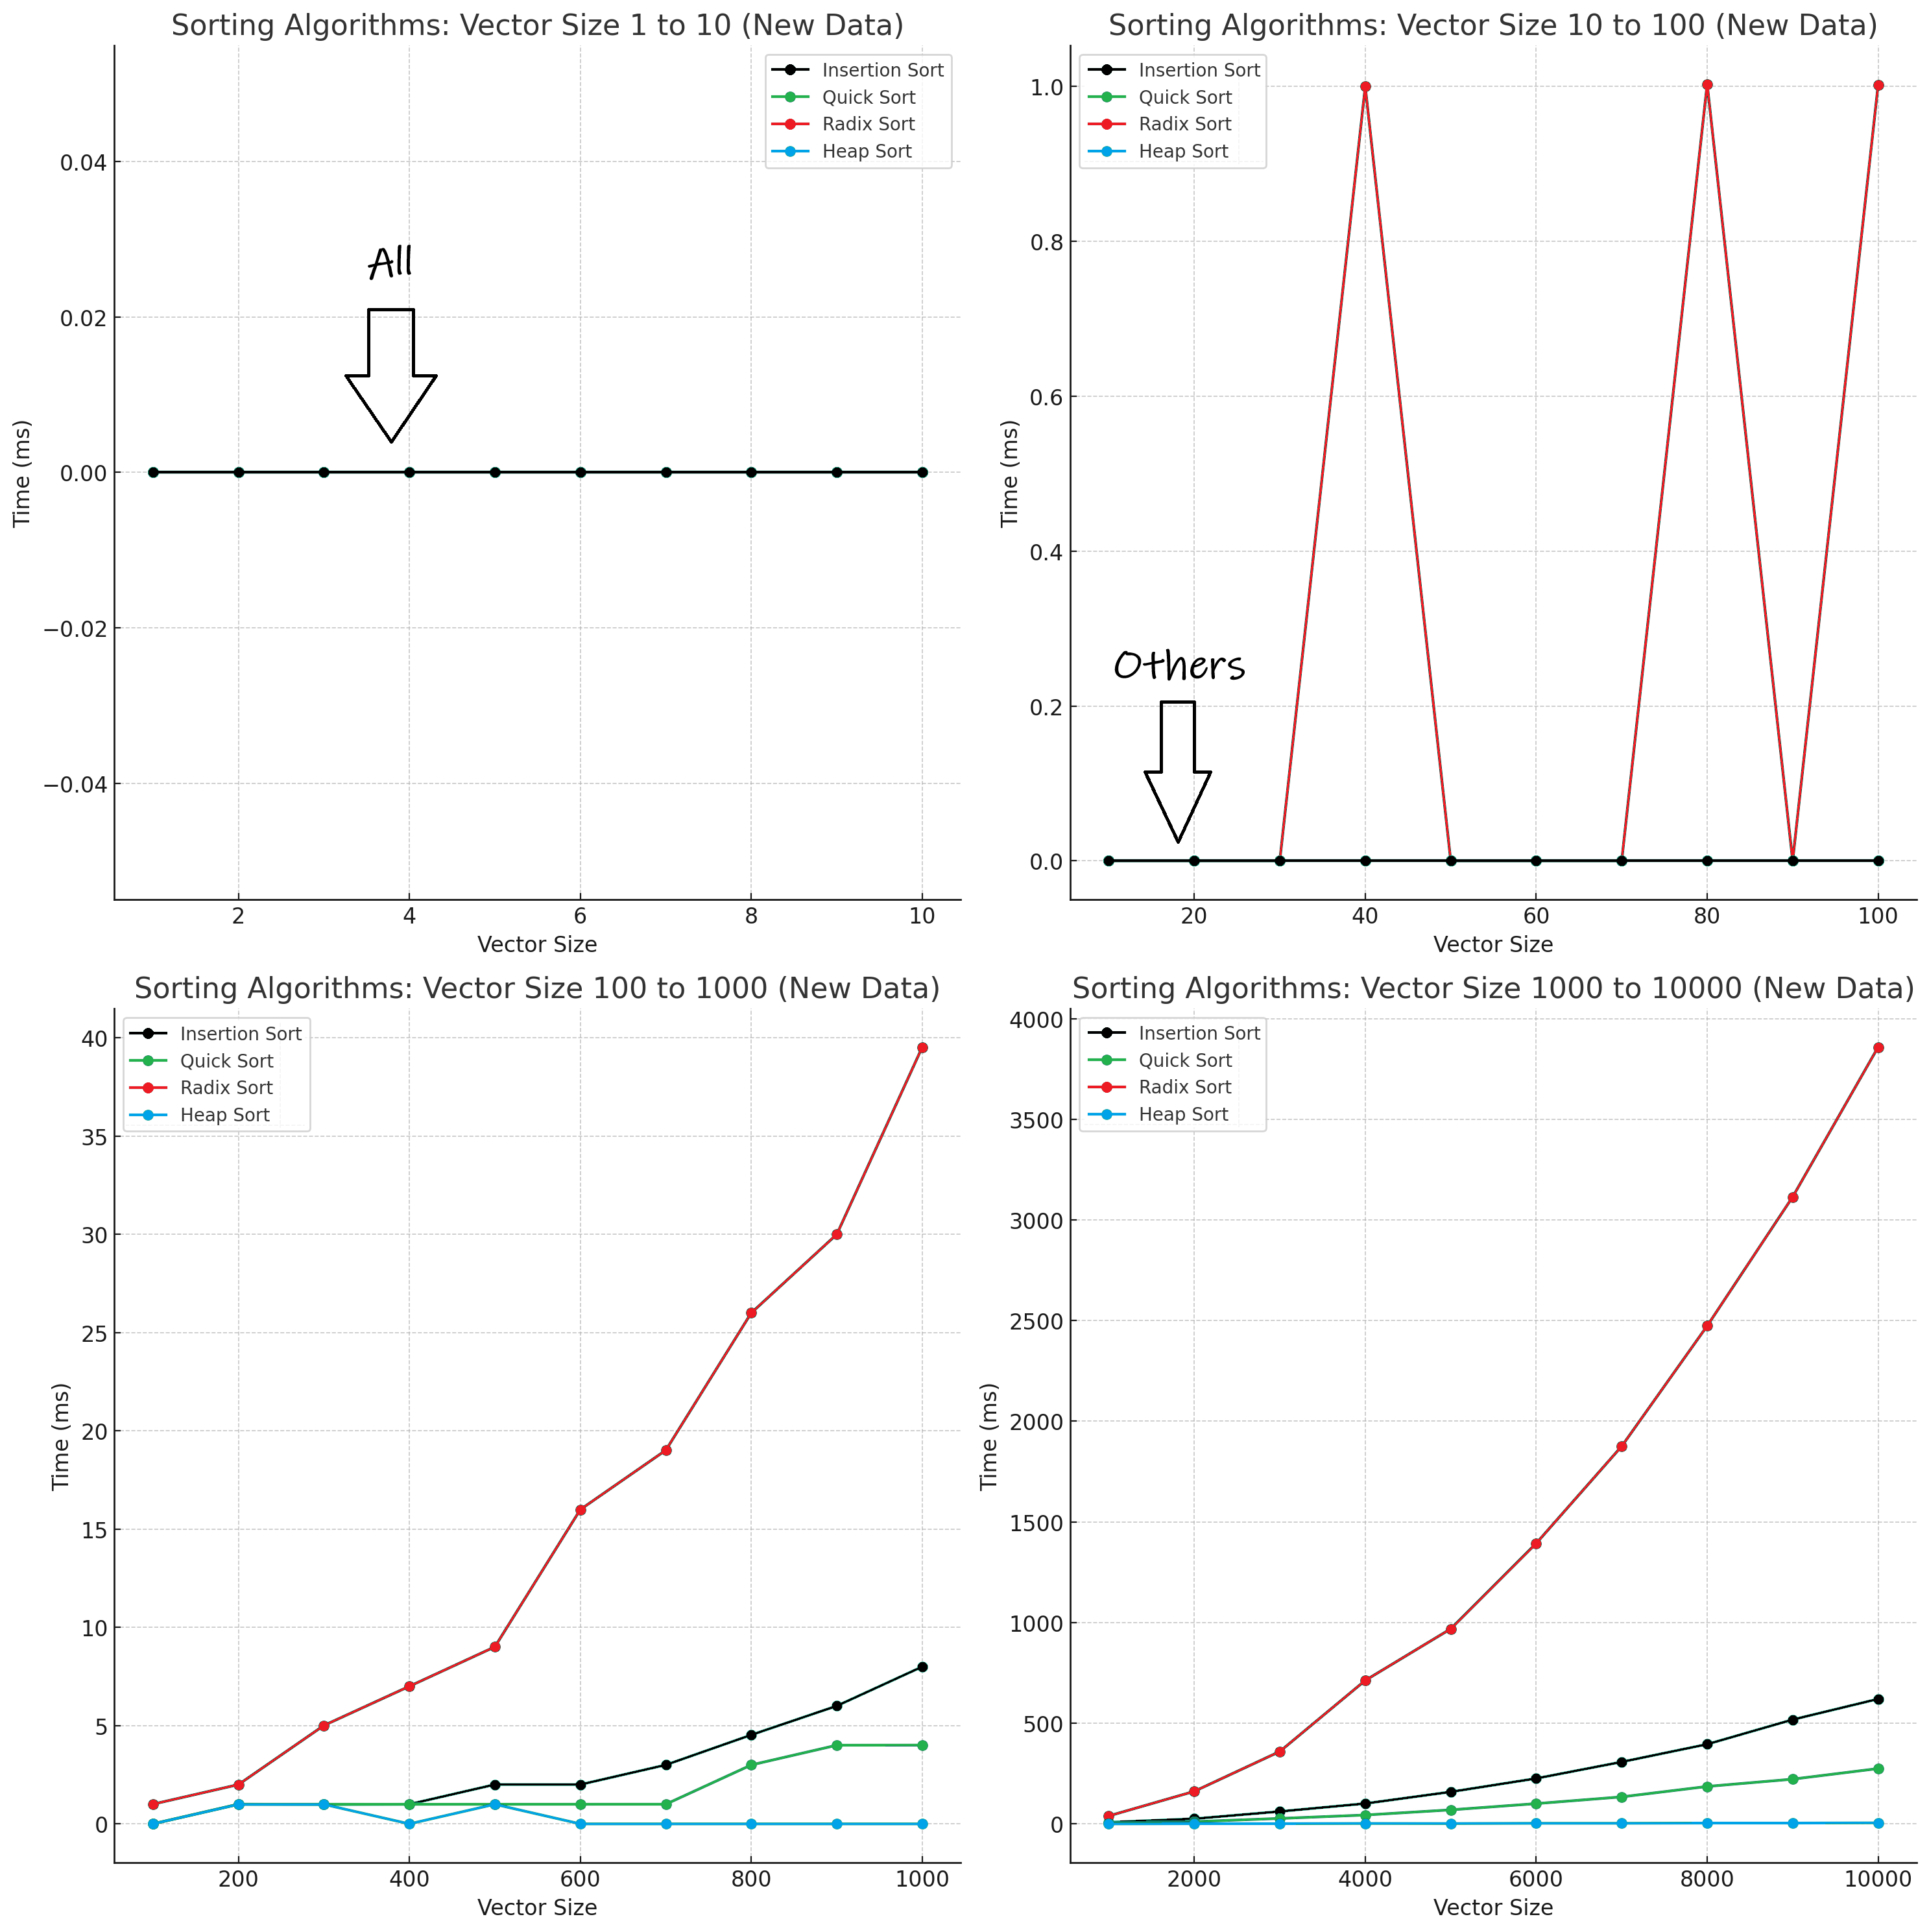
\includegraphics[width=1\linewidth,height=0.6\textheight]{../paper/full.png}
\caption* {The time each algorithm took to sort an array of randomly shuffled values.}
\end{figure}

Graphs of results for the average case of all sorting algorithms are presented in:
For size 0-10, (graphic 1) all sorting algorithms can work in 0ms.
For size 0-100, (graphic 2) occasionally, radix sort has minor time losses and other sorting algorithms can work in 0ms.
For size 0-1000 and 0-10000, (graphic 3-4) radix sort takes several times longer than the other sorting algorithms but heap sort takes the least time.

\section{Conclusions}

As a result, heap sort is best of the sorts, quick sort is second, insertion sort is third and radix sort is fourth one.


\end{document}
